

\section{Problem 1 - Computing moments}
Consider the following model for subject i in group h at time j:
 
\begin{align*}
	Y_{hij} &= \mu + \alpha_h + \beta_j + \gamma_{hj} + b_{hi} + \epsilon_{hij}
\end{align*}

where $b_{hi} \sim N(0, \sigma^2_b)$ and $\epsilon_{hij} \sim N(0, \sigma^2_e)$, for $h=1,..H, i=1,..n_h,$ and $j=1,.. J$. Assume that random variables that do not share a common value of h or i are independent. 

\begin{itemize}
\item[(a)] Compute $E[Y_{hij}]$.
	
	\begin{align*}
		Y_{hij} &= \mu + \alpha_h + \beta_j + \gamma_{hj} + b_{hi} + \epsilon_{hij} \\
		E[Y_{hij}] &= \mu + \alpha_h + \beta_j + \gamma_{hj} + E[b_{hi}] + E[\epsilon_{hij}] \\
		 E[b_{hi}] &= 0, \qquad E[\epsilon_{hij}] = 0, \qquad \text{as} \quad b_{hi} \sim N(0, \sigma^2_b), \epsilon_{hij} \sim N(0, \sigma^2_e) \\
		E[Y_{hij}] &= \mu + \alpha_h + \beta_j + \gamma_{hj} 
	\end{align*}

\item[(b)] Don't assume $b_{hi}$ and $\epsilon_{hij}$ are independent. Derive an expression for $Var[Y_{hij}]$ that it as simplified as possible.

If $b_{hi}$ and $\epsilon_{hij}$ are not independent,
\begin{align*}
	Var[b_{hi} + \epsilon_{hij}] &= Var[b_{hi}] + Var[\epsilon_{hij}] +2 Cov[b_{hi}, \epsilon_{hij}] \\
	Y_{hij} &= \mu + \alpha_h + \beta_j + \gamma_{hj} + b_{hi} + \epsilon_{hij} \\
	Var[Y_{hij}] &= Var[b_{hi} + \epsilon_{hij}] \\
	Var[b_{hi}] &= \sigma^2_b, \qquad Var[\epsilon_{hij}] = \sigma^2_e, \qquad \text{as} \quad b_{hi} \sim N(0, \sigma^2_b), \epsilon_{hij} \sim N(0, \sigma^2_e) \\
	Var[Y_{hij}] &= \sigma^2_b + \sigma^2_e + 2 Cov[b_{hi}, \epsilon_{hij}] \\
	&=  \sigma^2_b + \sigma^2_e + 2 \Bigg( E \Big[ b_{hi} \epsilon_{hij} \Big] - E[b_{hi} ] E[\epsilon_{hij}] \Bigg) \\
	&= \sigma^2_b + \sigma^2_e + 2 E \Big[ b_{hi} \epsilon_{hij} \Big] 
\end{align*}

\item[(c)] assume $b_{hi}$ and $\epsilon_{hij}$ are independent. Derive an expression for $Var[Y_{hij}]$. 

If $b_{hi}$ and $\epsilon_{hij}$ are independent,
\begin{align*}
	Cov[b_{hi}, \epsilon_{hij}] &= 0\\
	Var[Y_{hij}] &= \sigma^2_b + \sigma^2_e
\end{align*}

\end{itemize}

\section{Problem 2 - Correlation in Data}
Consider the general linear regression model:

\begin{align*}
	Y_{n \times 1} &= X_{n \times p} \beta + \epsilon_{n \times 1}
\end{align*}

where $\epsilon$ is normal, and $\theta$ is unknown.

\begin{itemize}
	\item [(a)] Show the the ordinary least squares (OLS) estimator $\hat{\beta}^{OLS}$ is unbiased.
	We need to show $E(\hat{\beta}^{OLS}) = \beta$
\begin{align*}
	\hat{\beta}^{OLS} &=  (X^T X)^{-1}X^T Y \\
	E(\hat{\beta}^{OLS}) &= (X^T X)^{-1}X^T E(Y) =  (X^T X)^{-1}X^T X \beta = \beta
\end{align*}	
	
	\item[(b)] Derive the variance of $\hat{\beta}^{OLS}$ 
	
\begin{align*}
	Var(\hat{\beta}^{OLS}) &= Var((X^T X)^{-1}X^T Y )= (X^T X)^{-1}X^T Var(Y) [(X^T X)^{-1}X^T ]^T \\
	Var(Y) &= \Sigma \\
	Var(\hat{\beta}^{OLS})  & =  (X^T X)^{-1}X^T \Sigma X [(X^T X)^{-1}] 
\end{align*}		
	if X is non-singular, we can further simplify 
\begin{align*}	
	Var(\hat{\beta}^{OLS})	&= X^{-1} (X^T)^{-1} X^T \Sigma X X^{-1} (X^T)^{-1} \\
	&= X^{-1} \Sigma (X^T)^{-1} = [X^T \Sigma^{-1} X]^{-1}
\end{align*}		
	
	\item[(c)] Derive an expression for the variance of $\hat{\beta}^{OLS}$ (simplified as much as possible).
	
	\begin{align*}
	\Sigma &= \sigma^2 I_{n \times n} \\
	Var(\hat{\beta}^{OLS}) &= [X^T \Sigma^{-1} X]^{-1} = \sigma^2 (X^T X)^{-1}
\end{align*}

\item[(d)] Now, assume n = 10, p = 1, and let X be a vector of ones (e.g., an intercept only model). $\rho in (0,1)$, plot the true standard deviation of $\hat{\beta}^{OLS}$ as a function of $\rho$.

\begin{align*}
	\Sigma &= \sigma^2 I_{n \times n} = \begin{pmatrix}
	1 & \rho &.. & \rho \\
	\rho & 1 &.. & \rho\\
	.. &.. & ..& \\
	\rho & \rho &. .& 1  
	\end{pmatrix}
\end{align*}

The plot of SD as a function of $\rho$ as below:
\begin{figure}[h]
	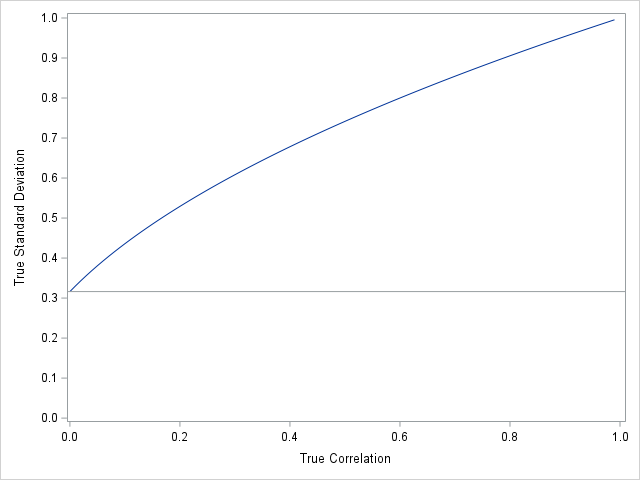
\includegraphics[width=15cm]{2d.png}
\end{figure}

The SAS codes are as below
\lstinputlisting[language=SAS]{HW1-Q2-PD.sas}


\item[(e)] From the previous example, as $\rho \rightarrow 1 $, you should observe that the true SD for $\hat{\beta}_{OLS} \rightarrow 1$. Concisely state why this is the case using one or two complete sentences.

From the SD formula, we calculate 
\begin{align*}
	\Sigma &= \begin{pmatrix}
		1 & \rho &.. & \rho \\
		\rho & 1 &.. & \rho\\
		.. &.. & ..& \\
		\rho & \rho ..&. & 1 
	\end{pmatrix} = \begin{pmatrix}
	1 & 1 &.. & 1 \\
	1 & 1 &.. & 1 \\
	.. &.. & ..& \\
	1 & 1 &. .& 1 
\end{pmatrix} , \qquad \rho \rightarrow 1\\
X &= (1,...1)^T,  X^T X = 10 \\
	Var(\hat{\beta}^{OLS}) & = (X^T X)^{-1}X^T \Sigma X [(X^T X)^{-1}] \\
	&= 10^{-1} (1,...1) \begin{pmatrix}
		1 & 1 &.. & 1 \\
		1 & 1 &.. & 1 \\
		.. &.. & ..& \\
		1 & 1 &. .& 1 
	\end{pmatrix} _{10 \times 10} (1,...1)^T 10^{-1} \\
&= 10^{-1} (10,...10) (1,...1)^T 10^{-1}  = 1\\
\end{align*}

When correlation coefficient is 1, we have the covariance is the same as variance, which shows that there is only one sample regression model. So the variance of the estimate $\hat{\beta}_{OLS}$ is the variance of response variable or error term, which is 1.

\item[(f)] Hypothesis test of $\beta$. They do so using the OLS estimator but erroneously assume independent covariance matrix. when in fact the correlation between observations$\rho = \frac{1}{n-1}$. Note that, in this case is equal to the sample mean. What is the actual type I error rate for this test? What can you say about the impact of ignoring even small positive correlation in ananalysis when the sample size is large?

When we erroneously assume independent covariance matrix, $\Sigma = I$, then 
\begin{align*}
	\hat{\beta}  &=  (X^T X)^{-1}X^T Y = \bar{Y}\\
	Var(\hat{\beta} ) &= (X^T X)^{-1}X^T I X [(X^T X)^{-1}] = (X^T X)^{-1} = \frac{1}{10}
\end{align*}

So the critical value 
\begin{align*}
	z &= \frac{\hat{\beta} }{\sqrt{Var(\hat{\beta})}}  =  \bar{Y} \sqrt{10}
\end{align*}

The rejection region with $1-\alpha \%$ CI is $z > Z_{1-\alpha/2}, z < Z_{-\alpha/2}$, under the independent covariance matrix.


While, when we assume correlation $\rho = \frac{1}{n-1}$, we have the corrected variance for $Var(\tilde{\beta} )$. 
\begin{align*}
	\hat{\beta}  &=  (X^T X)^{-1}X^T Y = \bar{Y}\\
	Var(\tilde{\beta} ) &= (X^T X)^{-1}X^T \Sigma X [(X^T X)^{-1}]  \\
	\Sigma &= \begin{pmatrix}
		1 & \rho &.. & \rho \\
		\rho & 1 &.. & \rho\\
		.. &.. & ..& \\
		\rho & \rho ..&. & 1 
	\end{pmatrix} = \begin{pmatrix}
		1 & \frac{1}{9} &.. & \frac{1}{9} \\
		\frac{1}{9}  & 1 &.. & \frac{1}{9} \\
		.. &.. & ..& \\
		\frac{1}{9}  & \frac{1}{9}  ..&. & 1 
	\end{pmatrix} \\
	Var(\tilde{\beta} ) &= \frac{1}{10} (1,1..1) \begin{pmatrix}
		1 & \frac{1}{9} &.. & \frac{1}{9} \\
		\frac{1}{9}  & 1 &.. & \frac{1}{9} \\
		.. &.. & ..& \\
		\frac{1}{9}  & \frac{1}{9}  ..&. & 1 
	\end{pmatrix} \\ (1,1..1)^T \frac{1}{10}  = \frac{1}{5}
\end{align*}

The actual variance of $\hat{\beta}$ is larger (1/5) than the variance assuming independent covariance (1/10). So the two sided rejection region will be smaller than the region based on incorrect covariance matrix. In other words, the type I error is inflated based on independent covariance matrix assumption.

The actual type I error rate based on independent covariance matrix assumption
\begin{align*}
	p(x > \hat{\beta} | \beta = 0) &= p(x <- \hat{\beta} |  \beta = 0) \\
	p &= 2 p(x> \hat{\beta} | \tilde{\beta}) = 2 p(\bar{Y} \sqrt{10} > z_{1-\alpha/2})
\end{align*}

We will use the below SAS codes to simulate the actual type I error rate, which is $ 0.16618$. 

The SAS codes are as below:
\lstinputlisting[language=SAS]{HW1-Q2-PE.sas}

Generalize the type I error rate 

\begin{align*}
	\alpha_0 &= 2p( \bar{Y} > Z_{1-\alpha/2} SD(\hat{\beta}) | \bar{Y} \sim N(0, Var(\tilde{\beta}))) \\
	&= 1 - p(\frac{Z_{1-\alpha/2} sd(\hat{\beta})}{sd(\tilde{\beta})}) + p(- \frac{Z_{1-\alpha/2} sd(\hat{\beta})}{sd(\tilde{\beta})})
\end{align*}

The variance of $\tilde{\beta}$
\begin{align*}
	Var(\tilde{\beta} ) &= (X^T X)^{-1}X^T \Sigma X [(X^T X)^{-1}]  \\
	\Sigma &= \begin{pmatrix}
		1 & \rho &.. & \rho \\
		\rho & 1 &.. & \rho\\
		.. &.. & ..& \\
		\rho & \rho ..&. & 1 
	\end{pmatrix} = \begin{pmatrix}
		1 & \frac{1}{n-1} &.. & \frac{1}{n-1} \\
		\frac{1}{n-1}  & 1 &.. & \frac{1}{n-1} \\
		.. &.. & ..& \\
		\frac{1}{n-1}  & \frac{1}{n-1}  ..&. & 1 
	\end{pmatrix} \\
	Var(\tilde{\beta} ) &= \frac{1}{n} (1,1..1)_{n \times 1} \begin{pmatrix}
		1 & \frac{1}{n-1} &.. & \frac{1}{n-1} \\
		\frac{1}{n-1}  & 1 &.. & \frac{1}{n-1} \\
		.. &.. & ..& \\
		\frac{1}{n-1}  & \frac{1}{n-1}  ..&. & 1 
	\end{pmatrix}  (1,1..1)^T_{1 \times n} \frac{1}{n}  = \frac{2}{n}
\end{align*}

So the generalized type I error rate is $1 - p(Z_{1-\alpha/2} \sqrt{2}) + p(- Z_{1-\alpha/2} \sqrt{2})$. We could see that the type I error rate doesn't change when sample size get larger.
Also we use the simulated codes as above and changed the sample size n, the type I error rate is almost the same. 
 
The plot of type I error rate vs. sample size as below:
\begin{figure}[h]
	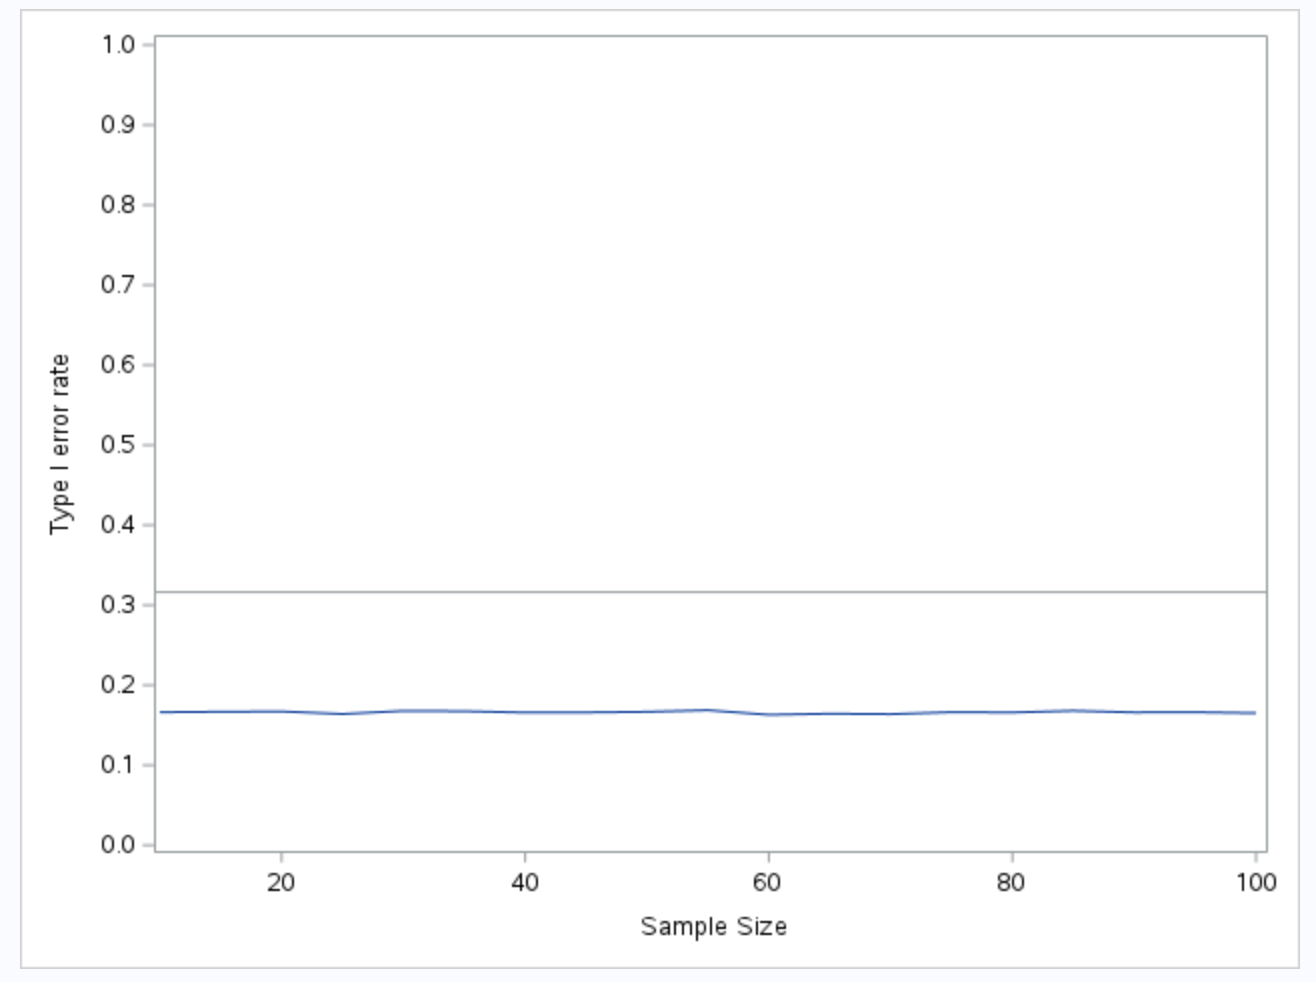
\includegraphics[width=10cm]{HW1-2b.png}
\end{figure}

The SAS codes for generating the above type I error rate figure as below:
\lstinputlisting[language=SAS]{BIOS767-hw1.sas}

\end{itemize}

\section{Problem 3- Naive approach to handle correlation in Data}

Consider the subject-specific linear regression model:
\begin{align*}
	Y_{hij}  &= \beta_{h0} + t_{hij} \beta_{h1} + \epsilon_{hij} \\
	\hat{\beta}_{hi} &= (\hat{\beta}_{hi,0}, \hat{\beta}_{hi,1})^T = (X_{hi}' X_{hi})^{-1} X_{hi}' Y_{hi}
\end{align*}
The analyst plans to test the hypotheses 
\begin{align*}
	H_0:   & \beta_{11} = \beta_{21} \qquad vs. \qquad H_1: \beta_{11} \neq \beta_{21}
\end{align*}
using a two-sample t-test using the values $\hat{\beta}_{hi,1}: h= 1,2 ; i= 1,..n $ 

\begin{itemize}[]
	
	\item[(a)] Compute $E[\hat{\beta}_{hi} ], Var[\hat{\beta}_{hi} ], Var[\hat{\beta}_{hi,1} ]$. 
\begin{align*}
		\hat{\beta}_{hi} &= (X_{hi}' X_{hi})^{-1} X_{hi}' Y_{hi} \\
	E(\hat{\beta}_{hi}) &= (X_{hi}' X_{hi})^{-1} X_{hi}' E[Y_{hi}] \\
	& =  (X_{hi}' X_{hi})^{-1} X_{hi}' X_{hi} \beta_{hi} =\beta_{hi} 
\end{align*}	

the variance 
\begin{align*}
	Var(\hat{\beta}_{hi}) &= Var \Big((X_{hi}' X_{hi})^{-1} X_{hi}' Y_{hi} \Big) \\
	&= (X_{hi}' X_{hi})^{-1} X_{hi}' Var(Y_{hi}) \Big[ (X_{hi}' X_{hi})^{-1} X_{hi}' \Big]^T \\
	Var(Y) &= Var(\epsilon_{hi})= \Sigma_{J_{hi} \times J_{hi}}\\
	Var(\hat{\beta}_{hi})  & =  (X_{hi}' X_{hi})^{-1} X_{hi}' \Sigma_{J_{hi} \times J_{hi}} \Big[ (X_{hi}' X_{hi})^{-1} X_{hi}' \Big]^T \\
	\hat{\beta}_{hi,1} &= e_i^T \hat{\beta}_{hi} \, \qquad e_i = (0,1)\\
	Var(\hat{\beta}_{hi,1}) &= Var \Big(e_i^T \hat{\beta}_{hi} \Big) = e_i^T  Var(\hat{\beta}_{hi}) e_i\\
&= (0,1) (X_{hi}' X_{hi})^{-1} X_{hi}' \Sigma_{J_{hi} \times J_{hi}} \Big[ (X_{hi}' X_{hi})^{-1} X_{hi}' \Big]^T  \begin{pmatrix}
	0 \\
	1
\end{pmatrix} 
\end{align*}		

\item[(ii)] Will the analyst's assumption of a common variance across the $\hat{\beta_{ji,1}}$ hold in general? It not, explain why not and give a sufficient condition such that the planned two-sample t-test's assumptions will hold.

From above, we have the variance of $\hat{\beta}_{hi,1}$, which is $(0,1) (X_{hi}' X_{hi})^{-1} X_{hi}' \Sigma_{J_{hi} \times J_{hi}} \Big[ (X_{hi}' X_{hi})^{-1} X_{hi}' \Big]^T  \begin{pmatrix}
	0 \\
	1
\end{pmatrix} $. 
The assumption of a common variance will require the $X_{hi}$ and $\Sigma_{J_{hi} \times J_{hi}} $ are the same from different individuals. However, in longitudinal study, the design matrix X varies across individuals as they will have different measurement time. Also the covariance matrix between different measurements may be different. While in reality, the assumption does not hold due to the heterogeneity among individuals.

The sufficient condition for using t-test is to have i.i.d. observations among different groups, which requires the common variances of $\hat{\beta_{ji,1}}$. So we will need the design matrix and covariance matrix are the same for the two groups population. 

\end{itemize}

